%%%%%%%%%%%%%%%%%%%%%%%%%%%%%%%%%%%%%%%%%%%%%%%%%%%%%%%%%%%%%%%%%%%%%%%%%%%%%%%%%
%
% name: ADAQAcquisition_UsersGuide.tex
% date: 10 Oct 14
% auth: Zach Hartwig
% mail: hartwig@psfc.mit.edu
% desc: Main LaTeX file for the ADAQAcquisition User's Guide
%
%%%%%%%%%%%%%%%%%%%%%%%%%%%%%%%%%%%%%%%%%%%%%%%%%%%%%%%%%%%%%%%%%%%%%%%%%%%%%%%%%

\documentclass{report}

\usepackage[margin=1.5in]{geometry}
\usepackage{calc}
\usepackage{graphicx}
\usepackage{amsmath}
\usepackage{amssymb}
\usepackage{units}
\usepackage{url}
\usepackage{textcomp}
\usepackage{listings}
\usepackage{fix-cm}
\usepackage{color}
\usepackage{hyperref}

\special{
  ! userdict begin /bop-hook{
    stroke
    gsave 220 170 translate
    55 rotate /Times-Roman findfont 250 scalefont setfont
    0 0 moveto 0.9 setgray (Draft) show grestore
  }def end
}

\definecolor{grey}{rgb}{0.5, 0.5, 0.5}

% Package to allow inclusion of C++ code
\lstset{language=bash,basicstyle=\footnotesize}

\newcommand{\ADAQ}{\textsc{ADAQAcquisition }}
\newcommand{\ROOT}{\textsc{ROOT }}
\newcommand{\CAEN}{\textsc{Caen }}
\newcommand{\GIT}{\textsc{Git }}
\newcommand{\BOOST}{\textsc{Boost }}

\newcommand{\purl}{\protect\url}

\title{\begin{center}\includegraphics[width=6in]{figures/AIMSLogo_BoldPastelColors}\end{center}
  \vspace{1.5cm}
  \fontsize{36}{36}\selectfont \textbf{ADAQAcquisition} \\
  \fontsize{20}{20}\selectfont \textbf{A}IMS \textbf{D}ata \textbf{A}c\textbf{Q}uisition System \\
  \vspace{1.0cm} \fontsize{36}{36}\selectfont \textbf{User's Guide} \\
  \vspace{0.5cm} \fontsize{12}{12}\selectfont Document revision: October 2014\\
  ADAQAcquisition version: 0.99.4 \\
  \vspace{2cm}}

\author{\fontsize{20}{20}\selectfont Zachary S. Hartwig \\
  \fontsize{12}{12} \selectfont Massachusetts Insitute of Technolog \\
  Department of Nuclear Science and Engineering \& \\
  Plasma Science and Fusion Center}

\date{}

\begin{document}

\maketitle  

\chapter{Introduction to ADAQAcquisition}
\label{chap:introdurction}

\ADAQ is a program that provides a powerful graphical user interface
(GUI) method for the interacting, programming, and acquiring digitized
waveform data using CAEN high voltage and acquisition hardware. It
provides the user with a full range of functionality, from high level
methods for accomplishing complex tasks all the way to reading/writing
individual registers on the hardware. In addition to a fully featured
digital oscilloscope and multichannel analyzer, the program provides
persistent storage of waveform data in compressed binary files for
offline analysis with its sister program (\texttt{ADAQAnalysis}),
publication ready graphical output of waveforms and spectra, and
control over VME high voltage, VME-USB/OpticalLink bridge, and pulser
boards.

\ADAQ is built upon two main dependencies. The first is the
\texttt{ADAQ} library. The \texttt{ADAQ} library is a custom library
developed to provide standardized, straightforward, and enhanced
control over CAEN hardware. The library is available as a C++ shared
object library and Python module, encapsulating all of the standard
CAEN libraries with wrappers and extending these libraries by adding
new features. The second dependency is the \ROOT toolkit, which
provides object-oriented framework for data analysis, persistent
storage, and GUI construction.

At present, \ADAQ is only supported and tested on Linux platforms,
although in principle, building on Mac should be fairly straightfoward
provided the user's environment is correctly configured.


\section{Purpose of the \ADAQ User's Guide}
\label{sec: overviewsoftware}

The purpose of this user's guide is to provide the user of \ADAQ with
the information required to:
\begin{enumerate}
\item{Retrieve the \ADAQ source code from its public \GIT repository}
\item{Understand the general layout and build system of the \ADAQ
  source code}
\item{Configure the user's environment and build the \ADAQ binary}
\item{Educate the user in all the features of \ADAQ}
\end{enumerate}

Detailed documentation on the \CAEN libraries can be found here:\\
\href{http://www.caen.it/csite/LibrarySearch.jsp}{http://www.caen.it/csite/LibrarySearch.jsp}\\

Documentation on the \ROOT toolkit can be found here:\\
\href{http://root.cern.ch/drupal/content/documentation}{http://root.cern.ch/drupal/content/documentation}\\

To achieve these goals, the remainder of this chapter describes the
external software dependencies required to build the \ADAQ source code
and run its programs. Chapter~\ref{chap:svn} provides instructions on
how to obtain the \ADAQ source from the \GIT repository and building
\texttt{ADAQAcquisitionRootGUI} from source, including configuring the user's
Linux environment and some notes on obtaining and building the
external software dependencies. Chapter~\ref{chap:overview} provides a
detailed guide to the \texttt{ADAQAcquisitionRootGUI} program, including full
textual descriptions of each graphical widget available to the user as
well as annotated graphics of various parts of the
program. Chapters~\ref{chap:tutorial1} and \ref{chap:tutorial2}
contain step-by-step tutorials that walk the user through some of the
most important features of the \texttt{ADAQAcquisitionRootGUI} program. Finally,
Chapter~\ref{chap:source} provides an overview of the
\texttt{ADAQAcquisitionRootGUI} source code to enable the ambitious user to add
his/her own improvements to the software.

    
\section{Software Dependencies}
\label{sec: dep}
This section briefly describes the external software dependencies
required to build and execute the \ADAQ source code.

\subsection{The CAEN libraries}
\label{sec: caendep}
CAEN distributes hardware drivers and C libraries in support of its
data acquisition system hardware. The following is a complete list of
the required CAEN libraries for \ADAQ. Note that the most up-to-date
version of the CAEN libraries and driver that \textit{have been
  successfully tested} with \ADAQ are listed in parenthesis next to the
library name:
\begin{enumerate}
\item{\textbf{CAENVMELib} (\textit{CAENVMELib-2.30}): provides a set
    of C functions that enable communication with the VME crate
    backplane and attached VME modules with the CAEN ``bridge'' modules,
    such as the VME-USB V1718 board.}
\item{\textbf{CAENComm} (\textit{CAENComm-1.02}): provides a set of
    relatively high-level C functions that mask the low-level details
    of communication with VME hardware via VME protocol, such as
    reading/writing registers and other common VME functionality.}
\item{\textbf{CAENDigitizer} (\textit{CAENDigitizer-1.31}): provides a
    set of relatively high-level C functions that mask the low-level
    details of communication with the CAEN family of
    digitizers. Explicitly meant for digitial data acquisition with
    CAEN sampling ADC (analog-to-digital) modules such as the V1720
    board.}
\item{\textbf{V1718 Linux Driver} (\textit{Version 0.9}): provides
  necessary Linux driver to interface with the VME-USB V1718
  board. Must be built from source and installed before using
  \texttt{ADAQAcquisitionRootGUI}.}
\end{enumerate}
The \CAEN dependencies listed above are provided as part of the \ADAQ
source code distribution for convenience and to ensure explicit
version of control of the various libraries.\\

\noindent
The \CAEN homepage: \purl{http://www.CAEN.com}\\

\subsection{The \ROOT toolkit}
\label{sec: rootdep}
\ROOT\ is a free (as in no cost), open-source, C++ object-oriented
data analysis toolkit that was originated at CERN but is now developed
and maintained by a worldwide collaboration across many scientific
fields, although it is primarily used in particle and nuclear physics.

While it was developed explicitly for handling massive data sets, it
is also incredibly useful for data analysis on a small scale,
providing powerful histogramming, fitting, graphical output, and GUI
generation. It also contains a diverse array of powerful data analysis
tools that are available as class objects that can be applied to any
data set of data regardless of size. \ROOT is also powerful because
the user can fold his or her own C++ code with the \ROOT class objects
to create highly dynamic and customized data analysis, using all of
the power of C++: the standard libraries, the \BOOST libraries,
etc. It is open-source, constantly improved and maintained, and there
is a dynamic user community available online.\\

\noindent
The \ROOT homepage: \purl{http://root.cern.ch/drupal/}\\

\noindent
The \textsc{ROOTTalk} users forum: \purl{http://root.cern.ch/phpBB2/}\\

\subsection{The \BOOST C++ libraries}
\label{sec: boostdep}
\BOOST is a set of free (as in no cost), open-source, peer-reviewed
portable C++ libraries that are incredibly powerful and diverse.
\BOOST can be thought of as a significant extension of the C++
Standard Libraries and is often a testing ground for a majority of the
code that eventually gets folded into C++ during technical reviews.\\

\noindent
The \BOOST homepage: \purl{http://www.boost.org}\\

\chapter{Building CyDAQ from the SVN Repository}
\label{chap:svn}
This chapter describes in detail the steps required to obtain the \ADAQ
source code from its SVN repository home and then build the \ADAQ
executables from source.

\section{Prerequisites}
\label{sec:prereqs}
Before building the \ADAQ source code, a number of dependencies must be
installed on the user's local system in order to ensure a successful
build of the \ADAQ source code. While the specific details of building
each of these dependencies is outside the scope of this manual, a few
notes are provided below. It should be noted that all required
software dependencies are already installed on the Ionetix server,
greatly accelerating the process of building and the using the \ADAQ
software.

\subsection{\ROOT}
If the user will be building \ADAQ on his/her local Linux machine, \ROOT
may be downloaded from the following location:
\purl{http://root.cern.ch/drupal/content/downloading-root}. The most
recent version of \ROOT that has been successfully tested with the \ADAQ
source code is version 5.32.01. While \ROOT binaries are available for
direct installation, it is preferable to build \ROOT from source code
to ensure perfect configuration to the user's local environment. The
user is recommended to download the appropriate tarball and then
follow the directions for installing \ROOT from source that can be
found here:
\purl{http://root.cern.ch/drupal/content/installing-root-source}

If the user will be building \ADAQ on the Ionetix server, \ROOT version
5.32.01 has already been installed in
\texttt{/usr/local/root/root\_v5.32.01}. To use this version of \ROOT,
the user needs to add the following lines to his/her \texttt{.bashrc}
file:
\begin{lstlisting}
  export ROOTSYS=/usr/local/root/root_v5.32.01/root
  export PATH=$ROOTSYS/bin:$PATH
  export LD_LIBRARY_PATH=$ROOTSYS/lib:$LD_LIBRARY_PATH
\end{lstlisting}
These environmental variables ensure that the user has full access to
the \ROOT binaries and libraries required to build and run the \ADAQ
source code.


\subsection{\texttt{Boost}}
If the user will be building \ADAQ on his/her local Linux machine, the
\BOOST C++ libraries can either be installed via the operating systems
package manager (\texttt{apt-get} on Ubuntu or \texttt{yum} on
Fedora/RedHat) or downloaded from the \BOOST homepage at
\purl{http://www.boost.org/}. The vast majority of \BOOST
functionality is conventiently provided by header files and therefore
does not require building from source; such is the case for the parts
of \BOOST used by \ADAQ. The user can follow directions for installation
of the most recent \BOOST release (1.49.0) on Linux machines here:
\purl{http://www.boost.org/doc/libs/1_49_0/more/getting_started/unix-variants.html}

if the user will be building \ADAQ on the Ionetix server, \texttt{Boost}
is already installed at \texttt{/usr/include/boost}. No special action
is required of the user; \texttt{Boost} is ready to be used.


\section{Getting the \ADAQ source code}
\label{sec:sourcecode}
The \ADAQ source lives permanently in a Subversion code management
repository on the Ionetic Linux server \footnote{For the uninitiated,
  a good code management system is a highly scalable piece of software
  that allows developers to efficiently, seamlessly, and confidently
  work on a software project together with the full history of
  everyone's changes to the project (as well as all of the original
  files) fully documented and accessible at any time. They are
  incredibly useful for a developers or even just a single developer,
  if for nothing other than to document all changes and provide the
  ability to go back to any version of any file at any time.}. While
anyone with a user account on the Ionetix Linux server may check out a
working copy of the code, only users who are in the ``CyDAQ'' group
have permission to check in changes to the repository. To be added to
the CyDAQ developers group, please contact the author at
\texttt{hartwig@psfc.mit.edu}.

Checking out a copy of the source code depends on the location from
which you connecting to the SVN repository: a ``local'' connection
refers to a user who is logged into and working on the Ionetix server;
a ``remote'' connection refers to a user who is working on a remote
computer with SSH capababilites that is running Subversion.\\

\noindent
To checkout a copy of the \ADAQ source code \textit{locally}, the user
should open a terminal on the Ionetix server and type:
\begin{lstlisting}
  svn co file:///usr/local/svn_repos/__CYDAQ_REPO__ /path/to/checkout
\end{lstlisting}
where the user should replace \texttt{/path/to/checkout} with the
directory
he/she would like SVN to place the checked out \ADAQ source code.\\

\noindent
To checkout a copy of the \ADAQ source code \textit{remotely}, the user
should open a terminal on his/her local machine and type:
\begin{lstlisting}
  svn co svn+ssh://username@ipaddress/usr/local/svn_repos/__CYDAQ_REPO__ /path/to/checkout
\end{lstlisting}
where the user should replace \texttt{username} with his/her username
on the Ionetix server, \texttt{ipaddress} with the IP address of the
Ionetix server, and /path/to/checkout with the directory on the
user's local machine that he/she would like SVN to place the checked
out \ADAQ source code.

\section{Overview of \ADAQ directory structure}
\label{sec:directorystructure}
After checking out the \ADAQ source code from the SVN repository as
described in Section~\ref{sec:sourcecode}, navigate to the top-level
\ADAQ directory, which will be the path specified to SVN when the copy
of the source code was checked our of the repository
(/path/to/checkout in the directions above). This directory is known
as the top-level directory. The directory and file structure below
this directory is descibed below:

\begin{itemize}
  \item{\textbf{analysis/}: contains a ``template'' for offline data
    analysis of digitized waveforms produced with
    \texttt{CyDAQRootGUI}. Designed to show the user how to access
    stored waveforms and provide a basis for his/her own analysis
    code.}
  \item{\textbf{manual/}: contains all of the files (\LaTeX files,
    images files in the images/ subdirectory, and the GNUmakefile for
    creating the beautiful manual you are now reading.}
  \item{\textbf{source/}: contains the bulk of the \ADAQ source
    code. The \textbf{versions/} subdirectory (empty as present) will
    contain snapshots of the \ADAQ source. The snapshots will be
    versioned and used when acquiring mission critical data, such that
    the state of the \ADAQ source code can be linked to experimental
    data sessions. The \textbf{trunk/} subdirectory contains the
    \texttt{CyDAQRootGUI} source code in subdirectories and the GNU
    makefile:
    \begin{itemize}
      \item{\textbf{bin/}: contains the \texttt{CyDAQRootGUI} binary
        after building via the GNU makefile. Other useful binaries are
        also in this directory.}
      \item{\textbf{build/}: a dumping ground for transient files
        created during the build process. The files are source code
        object files and \ROOT dictionary files.}
      \item{\textbf{include/}: C++ header files for
        \texttt{CyDAQRootGUI}.}
      \item{\textbf{lib/}: CAEN libraries required to build and run
        \texttt{CyDAQRootGUI}. The purpose of including these
        libraries here (rather than relying on installed CAEN
        libraries in places like /usr/lib) is for portability and to
        maintain explicit control over the versioning of CAEN
        libraries. The CAEN libraries are evolving and only somewhat
        decently documented, so it is important to ensure the correct
        versions of the libraries are used. Subdirectories contain
        libraries and soft links for both 32- and 64-bit architectures
        in the \textbf{x86/} and \textbf{x86\_64/} subdirectories.}
      \item{\textbf{src/}: C++ source code for \texttt{CyDAQRootGUI}.}
    \end{itemize}
  }
  \item{\textbf{utilities/}: contains some useful Python scripts.}
\end{itemize}

With the \ADAQ source code checked out and a basic understanding of the
source code structure, it's time to build the \texttt{CyDAQRootGUI}
binary.

    
\section{Configuring your environment}
\label{sec:config}
The \ADAQ source requires several environmental variables to be defined
in order to build and run correctly.
\begin{itemize}
\item{\textbf{CYDAQHOME}: Used by the \ADAQ GNU makefiles to determine
    the full paths to a number of source files and libraries. The
    value should be set as the full path to the top level of the \ADAQ
    source code.}
\item{\textbf{HOSTTYPE}: Used by the \ADAQ GNU makefiles to build the
    \ADAQ software tools for the correct architecture. The value should
    be set to ``x86'' for 32-bit architecture and ``x86\_64'' for
    64-bit architectures.}
\item{\textbf{PATH}: The Linux environmental variable that contains
    directories that are searched to determine the location of
    binaries. The bin directory for CyDAQRootGUI should be added to
    the \texttt{PATH} variable.}
\item{\textbf{LD\_LIBRARY\_PATH}: The Linux environmental variables that
    contains directories that are searched for dynamically linked
    libraries. The \ADAQ source code contains most of the required
    libraries for both 32- and 64-bit architectures. The lib directory
    for CyDAQRootGUI should be added to the \texttt{LD\_LIBRARY\_PATH}
    variable.}
\end{itemize}

The easiest way to set these four variables is to add the required
lines to the user's \texttt{.bashrc} file (which exists in his/her
home directory). For example, consider that user \texttt{zaphod} has
checked out a copy of the \ADAQ source code to the directory
\texttt{/home/zaphod/CyDAQ\_CheckOut} of the Ionetix server, which runs
a 64-bit operating system. He would need to add the following lines to
the file \texttt{/home/zaphod/.bashrc}:
\begin{lstlisting}
  export CYDAQHOME = /home/zaphod/CyDAQ_CheckOut
  export PATH = $CYDAQHOME/source/trunk/bin:$PATH
  export HOSTTYPE = x86_64
  export LD_LIBRARY_PATH = $CYDAQHOME/source/trunk/lib/$HOSTTYPE:$LD_LIBRARY_PATH
  $
\end{lstlisting}
\noindent
After these lines are added to the \texttt{.bashrc} file, the user
will either need to source the file in the currently open terminal or
simply close the terminal window and reopen a new one for the
environmental variables to take effect.

\section{Building the \texttt{CyDAQRootGUI} binary}
After ensuring that the prequisites described in
Section~\ref{sec:prereqs} have been successfully installed and
that the user's environment is configured as described in
Section~\ref{sec:config}, the user is ready to build the
\texttt{CyDAQRootGUI} binary.
\begin{itemize}
\item{Navigate to the \texttt{CyDAQRootGUI} directory:
    \begin{lstlisting}
      cd CYDAQHOME/source/trunk
    \end{lstlisting}
  }
\item{Build the binary from the source code using the provided GNU
    makefile:
    \begin{lstlisting}
      make
    \end{lstlisting}
    The GNU makefill will show the compilation steps and update the
    user on the progress of the build.
  }
\item{If successful, a new executable binary named
    \texttt{CyDAQRootGUI} should exist in the
    \texttt{\$CYDAQHOME/source/trunk/bin} directory
  }
\end{itemize}
That's all it takes! The user is now ready to begin running the
\texttt{CyDAQRootGUI} and should proceed to Chapter~\ref{chap:run}.

\chapter{An overview of \ADAQ}
\label{chap:overview}
This chapter gives a detailed overview of the \ADAQ
program, which provides a rich, graphical environment for simple but
powerful control over the entire data acquisition system. The user
will find directions to start the program, as well as complete textual
descriptions of each widget's functions and inputs. Annotated images
of the various frames of \ADAQ to demonstrate the
layout and location of all the widgets is also provided.

\section{Getting started}
\label{sec:start}
Because the directory containing the \ADAQ binary
should be in the user's \texttt{PATH} environmental variable (See
Section~\ref{sec:config}), the user may simply type:
\begin{lstlisting}
  CyDAQRootGUI
\end{lstlisting}
from any directory to start the program. Note that the directory from
which the user chooses to execute CyDAQRootGUI will, by default,
receive any output files (data files, graphic files) that the user
produces while running the program. Therefore, the user should at
least ensure that they have write access to the execution directory.
If all goes well, the program GUI should appear on the screen.


\section{Description of \ADAQ widgets}
This section contains detailed textual and graphical descriptions of
the widgets contained in the program.\ADAQ is divided
into three main windows, or ``frames'', with labelled tabs appearing
in the upper-left corner of the main \ADAQ window. The
user may switch to a particular frame by clicking on the associated
tab. Each main frame contains functionality that is logically grouped
under the appropriate tab heading. The following subsections describe
each widget contained on the main frames in detail and visually show
the main layout of each frame.


\subsection{The VMEConnection Frame}
The VMEConnection frame contains basic VME interaction functions, such
as establishing a VME connection to the VME boards, setting the VME
boards addresses in VME space, as well as reading/writing individual
registers from the V1720 and V6534 boards. An annotated view of the
VMEConnection frame appears in Figure~\ref{fig:vmeconnectionframe}

The following list contains a description of the function and input
required for each widget that appears on the VMEConnection frame:
\begin{itemize}
\item{\textbf{Connect/Disconnect button}: a large rectangular button
    that appears at the top-center of the frame initially as
    red. Clicking the button will attempt to connect to the V1720 and
    V6534 VME boards at the VME address specified in each board's VME
    address widget. If the connection is successful, the button will
    turn green and the text will indicate that the VME connection has
    been established. Clicking the button while the connection is
    estblished (the button is green) will then attempt to close the
    VME connection, returning the button color to red and setting the
    text to indicate the VME connectinon has successfully closed.}
  \item{\textbf{V6534BaseAddress number entry}: The 32-bit address of
      the V6534 board in VME space must be entered as an 8 digit hex
      number, with the first 4 hex digits corresponding to the VME
      address potentiometer settings on the physical V6534 board.}
  \item{\textbf{V6534 Read Cycle}: widgets that are used to manually
      read a single 16-bit value from one of the registers on the
      V6534 board and display it for inspection.
      \begin{itemize}
      \item{\textbf{Offset address number entry}: a 4 digit hex number
          describing the V6534 register address from which the
          register's value will be read.}
      \item{\textbf{Value}: the value stored at the register address
          specified in the address number entry above}
      \item{\textbf{VME read button}: initiate the VME read cycle to
          obtain the value from the V6534 register address specified
          in the address number entry above.}
      \end{itemize}
    }
  \item{\textbf{V6534 Write Cycle}: widgets that are used to manually
      write a single 16-bit value to one of the registers on the V6534
      board. Error checking is performed internally to prevent
      overwriting restricted registers.
      \begin{itemize}
      \item{\textbf{Offset address number entry}: a 4 digit hex number
          describing the V6534 register address to which the
          register's value will be written.}
      \item{\textbf{Value}: the value that will be written to the address
          specified in the address number entry above}
      \item{\textbf{VME read button}: initiate the VME write cycle to
          write the value to the V6534 register address specified in
          the address number entry above.}
      \end{itemize}
    }
  \item{\textbf{V1720BaseAddress number entry}: The 32-bit address of
    the V1720 board in VME space must be entered as an 8 digit hex
    number, with the first 4 hex digits corresponding to the VME
    address potentiometer settings on the physical V1720 board. It
    should be noted that if the user desires to use the CAEN DT5720
    desktop digitizer in place of the V1720 board then the VME address
    should be set to 0x00000000. The DT5720 should then be connected
    directly to the Ionetix server via the USB cable, bypassing the
    VME8100 crate and V1718 USB-VME board completely.}
  \item{\textbf{V1720 Read Cycle}: widgets that are used to manually
      read a single 32-bit value from one of the registers on the
      V1720 board and display it for inspection.
      \begin{itemize}
      \item{\textbf{Offset address number entry}: a 4 digit hex number
          describing the V1720 register address from which the
          register's value will be read.}
      \item{\textbf{Value}: the value stored at the register address
          specified in the address number entry above}
      \item{\textbf{VME read button}: initiate the VME read cycle to
          obtain the value from the V1720 register address specified
          in the address number entry above.}
      \end{itemize}
    }
  \item{\textbf{V1720 Write Cycle}: widgets that are used to manually
      write a single 32-bit value to one of the registers on the V1720
      board. Error checking is performed internally to prevent
      overwriting restricted registers.
      \begin{itemize}
      \item{\textbf{Offset address number entry}: a 4 digit hex number
          describing the V1720 register address to which the
          register's value will be written.}
      \item{\textbf{Value}: the value that will be written to the address
          specified in the address number entry above}
      \item{\textbf{VME read button}: initiate the VME write cycle to
          write the value to the V1720 register address specified in
          the address number entry above.}
      \end{itemize}
    }
\end{itemize}

\begin{figure}[b]
  \centering
  \caption{The VMEConnection frame as it appears in
    \ADAQ with annotations describing the general
    purpose of the containe widgets.}
  \label{fig:vmeconnectionframe}
  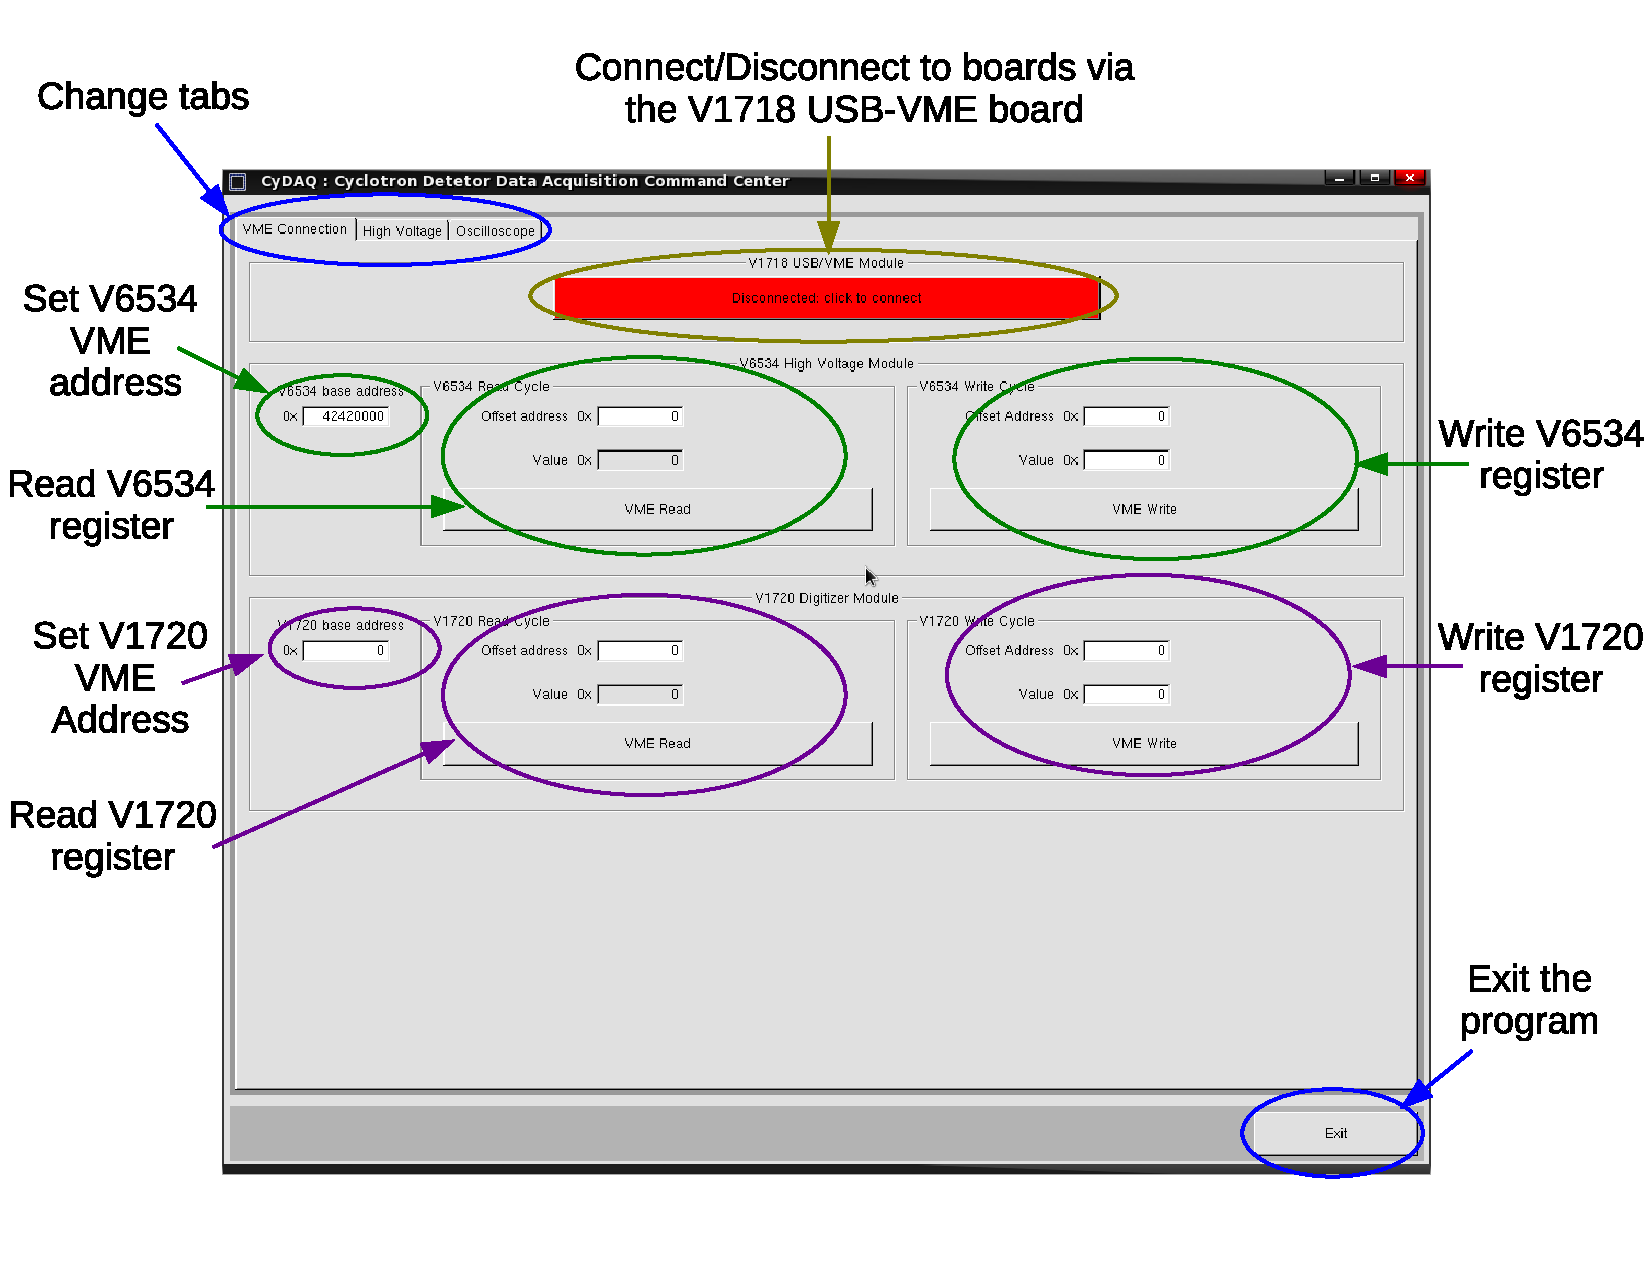
\includegraphics[width=6in]{images/VMEConnectionFrame}
\end{figure}

\subsection{The High Voltage Frame}
The High Voltage frame provides full control over the settings of the
V6534 high voltage board, including the voltage, current, and power
settings for each of the 6 channels. Real-time monitoring of set
voltage, drawn current, and power state (``on'' or ``off'') is
provided. An annotated view of the High Voltage frame appears in
Figure~\ref{fig:highvoltageframe}.

\begin{itemize}
\item{\textbf{High voltage settings for Channels 0--6}: There are 6
  identical ``group frames'' (with the exception of the V6534 channel
  they refer to as indicated by their label) that encapsulate the
  widgets for control of each channel's high voltage settings. 

  At present, a channel's set voltage and maximum drawn current can be
  set only while the channel is powered off, i.e. ``live'' changes to
  the voltage and current settings are not allowed. To modify an
  energized channel's voltage and current, the user must power the
  channel off, reset the voltage and current levels, and then power
  the channel back up. Automatic disabling the of voltage and current
  number entry widgets when a channel is energized enforce this
  standard. In the future, real-time adjustments of a channel's
  voltage and current while the channel is energized may be enabled.
    \begin{itemize}
    \item{\textbf{Set Voltage number entry}: the channel's voltage
        setting. Valid integer values are between 0 and 6000. Units of
        the number entry are in volts (V).}
    \item{\textbf{Set Current number entry}: the channel's maximum
        allowed drawn current. If more current is drawn that is set in
        this widget, the channel will trip off. Valid integer values
        are between 0 and 1000. Units of the number entry are in
        microamps ($\mu$A).}
    \item{\textbf{Active Voltage and Active Current number displays}:
        Disabled number entry widgets to the right of the ``Set''
        number entry widgets that display the channel's current set
        voltage and drawn current when the ``Enable monitoring'' check
        button is set (See below).}
    \item{\textbf{ON/OFF power button}: Button to the right of the
      channel set and display numebr entries. Button is red and marked
      ``OFF'' when the channel power state is ``OFF''. When clicked,
      the button will turn ``green'' and the text will be changed to
      ``ON'' to indicate that the channel has been energized. Note
      that the voltage/current ramp up and down relatively slowly and
      changes }
    \end{itemize}
  }
\item{\textbf{Enable Monitoring check box}: When this button is
    checked, the present values of active voltage and drawn current
    for all 6 channels are displayed in the ``Active Voltage'' and
    ``Active Current'' disabled number entry widgets for each
    channel. Updates are provided every 1 second.}
\end{itemize}

\begin{figure}
  \centering
  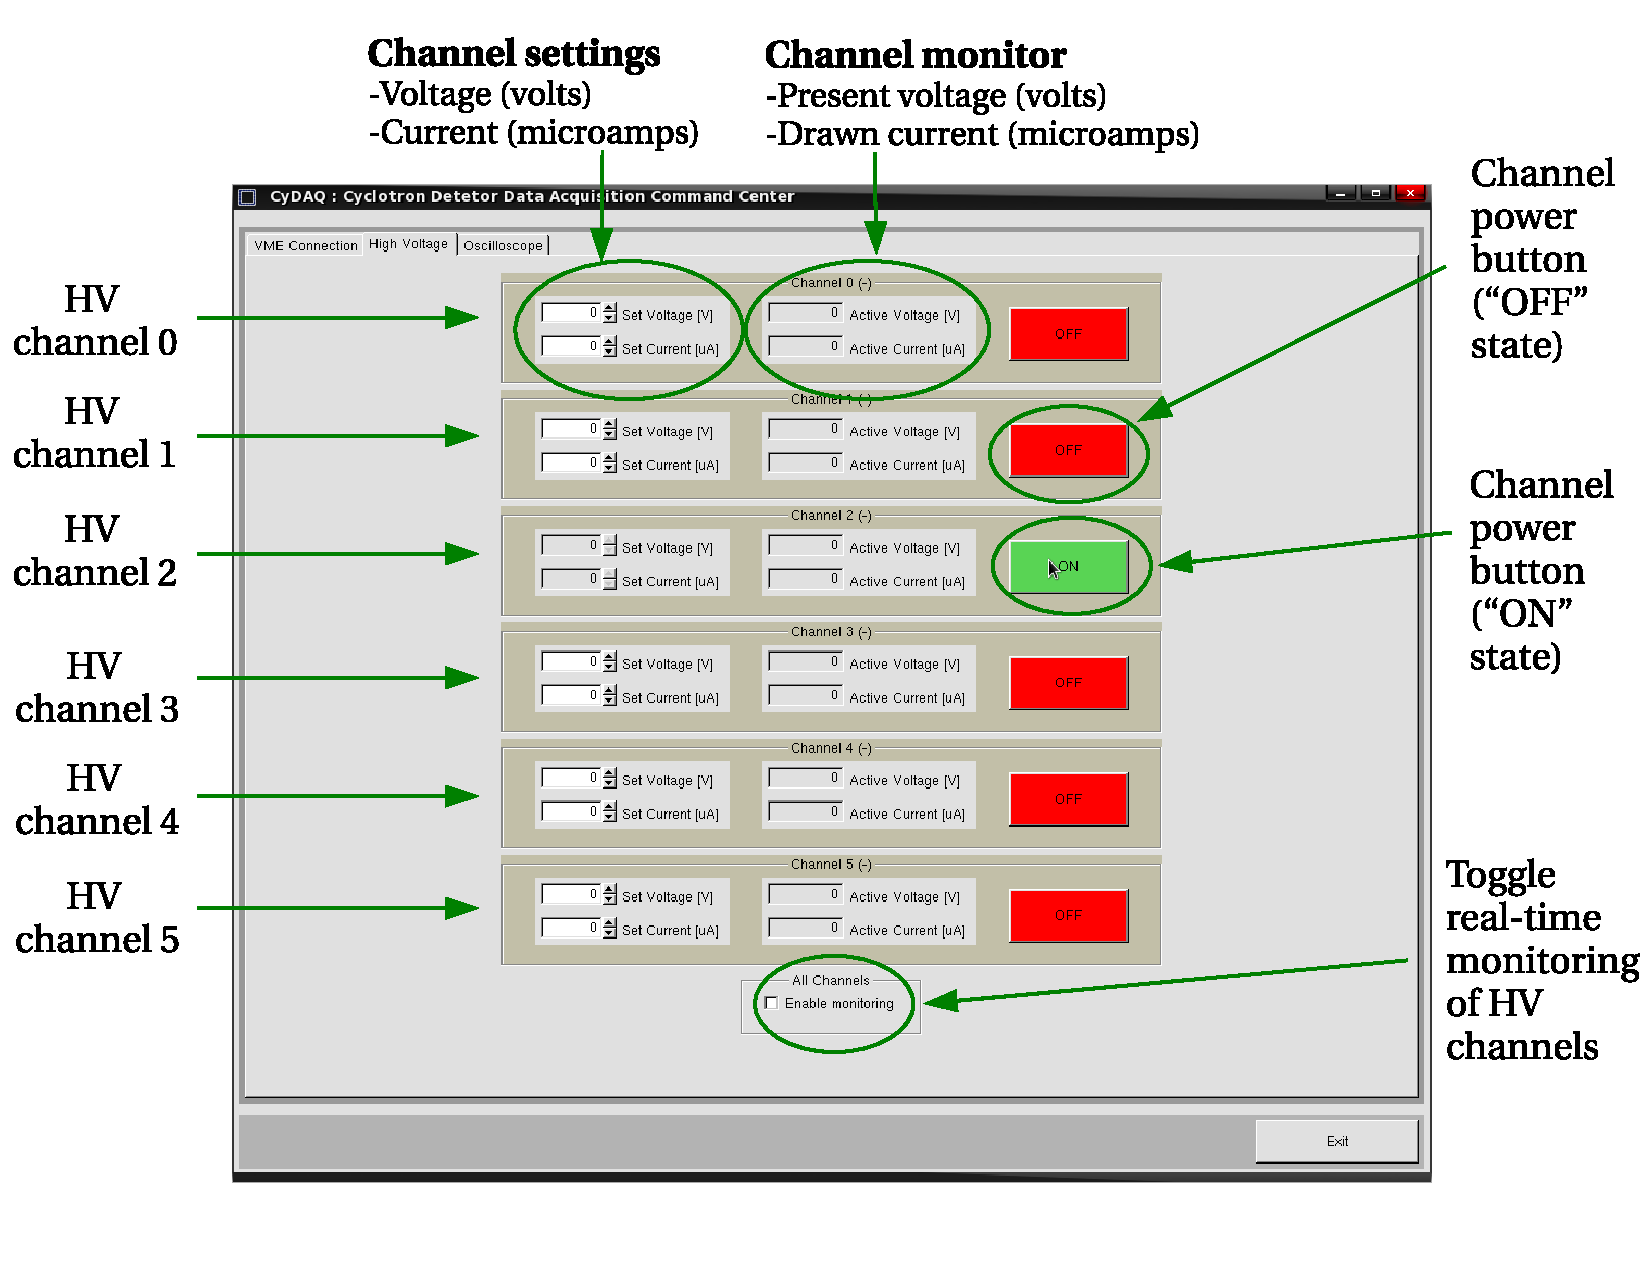
\includegraphics[width=6in]{images/HighVoltageFrame}
  \caption{The High Voltage frame as it appears in
    \ADAQ with annotations describing the layout and
    purpose of the encapsulated widgets.}
  \label{fig:highvoltageframe}
\end{figure}

\subsection{The Oscilloscope frame}
The Oscilloscope frame contains the powerful core of the
\ADAQ binary. Much more than the simple oscilloscope
the frame name implies, this frame contains a full feature digital
oscilloscope, widely configurable multichannel analyzer, graphical
plotter, and persistent data storage engine. The term ``DGScope''
(digitizer scope) is used to describe this powerful analysis tool. An
annotated view of the entire Oscilloscope frame appears in
Figure~\ref{fig:oscilloscopeframe}, while close-up views of the
important subframes appear in
Figures~\ref{fig:channel}--\ref{fig:datasubframe}.

The Oscilloscope frame is broadly divided into three main
subframes. The narrow, vertical subframe (the ``channel subframe'') at
the leftmost side of the main frame contains 8 group frames
(corresponding to the 8 V1720 digitizer channels).  Each group frame
(labelled by channel number from 0 to 7) contains 7 widgets that
control channel-specific settings. A scroll bar is provided at the
right of the subframeis provided to access to all 8 group frames and
their encapsulated widgets. An annotated picture of a single channel
group frame containing 7 channel-specific widgets appears in
Figure~\ref{fig:channel}.

The large, almost square subframe (the ``canvas subframe'') at the
top-right of the main frame contains four widgets: a large canvas for
plotting digitized waveforms and pulse spectra; a double vertical
slider for Y axis zoom control; a triple vertical slider for X axis
zoom control and calibration; and a large, red button labelled
``Stopped'' by default for starting/stopping data acquisition. The
canvas subframe can be easily seen in Figure~\ref{fig:oscilloscope}.

The final subframe (the ``scope subframe'') sits underneath the canvas
subframe at the bottom-right of the main Oscilloscope frame. The scope
subframe holds 4 tabbed subsubframes (Thins are etting complicated, I
know...), all of which hold widgets that apply general settings of the
DGScope: global scope function settings, pulse spectrum settings,
graphical settings, and data settings. Annotated pictures of each of
the 4 tabbed subsubframes can be seen in
Figures~\ref{fig:scopesubframe}--\ref{fig:datasubframe}

\begin{figure}
  \centering
  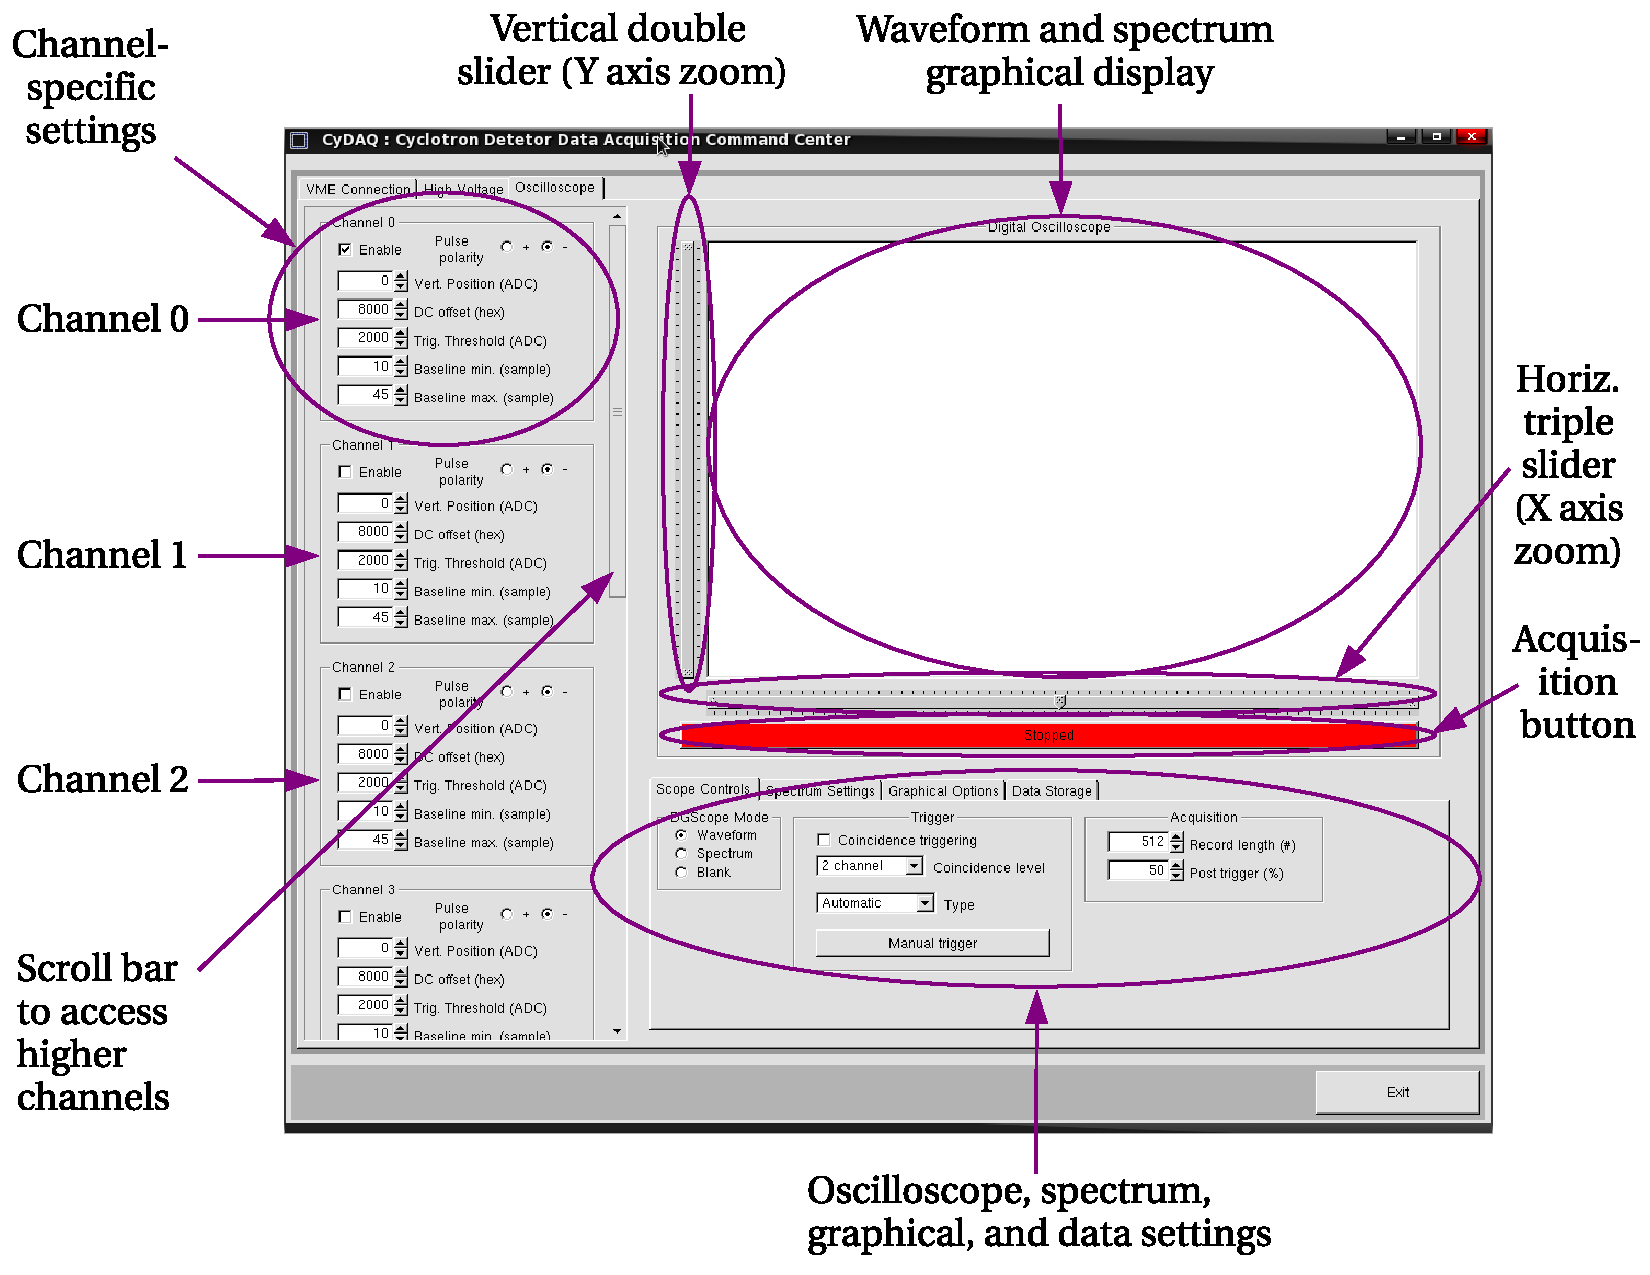
\includegraphics[width=6in]{images/OscilloscopeFrame}
  \caption{The Oscilloscope frame as it appears in
    \ADAQ with annotations describing the general
    purpose of the contained widgets.}
  \label{fig:oscilloscopeframe}
\end{figure}

\begin{figure}
  \centering
  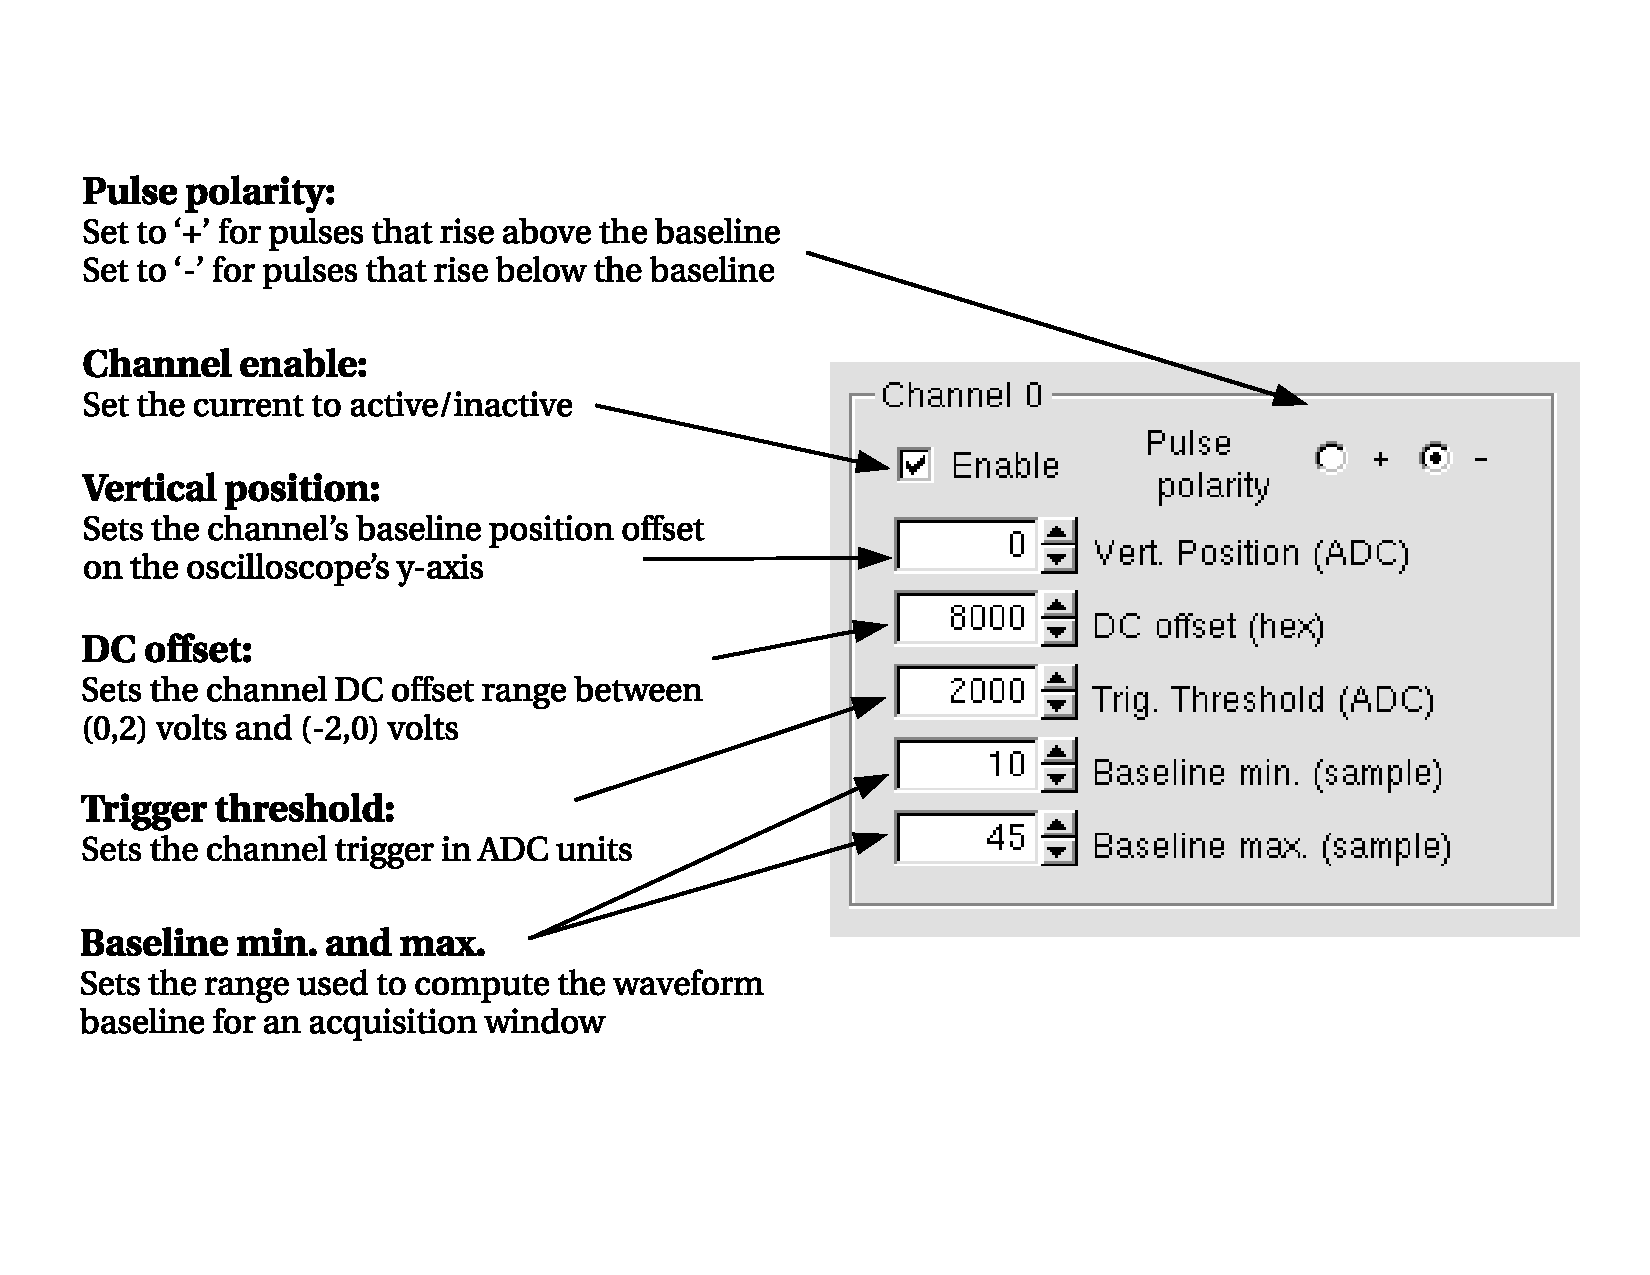
\includegraphics[width=6in]{images/OscilloscopeChannel}
  \caption{An annotated close-up view of one of the eight channel
    setting subframes contained in the Oscilloscope frame. In this
    example, each visible widget controls the channel-specific
    settings for the V1720 digitizer channel 0. A scroll bar is
    provided on the Oscilloscope frame to enable the user full access to
    all eight of the channel-specific setting subframes without
    hampering visibility and usability.}
  \label{fig:channel}
\end{figure}

\begin{figure}
  \centering
  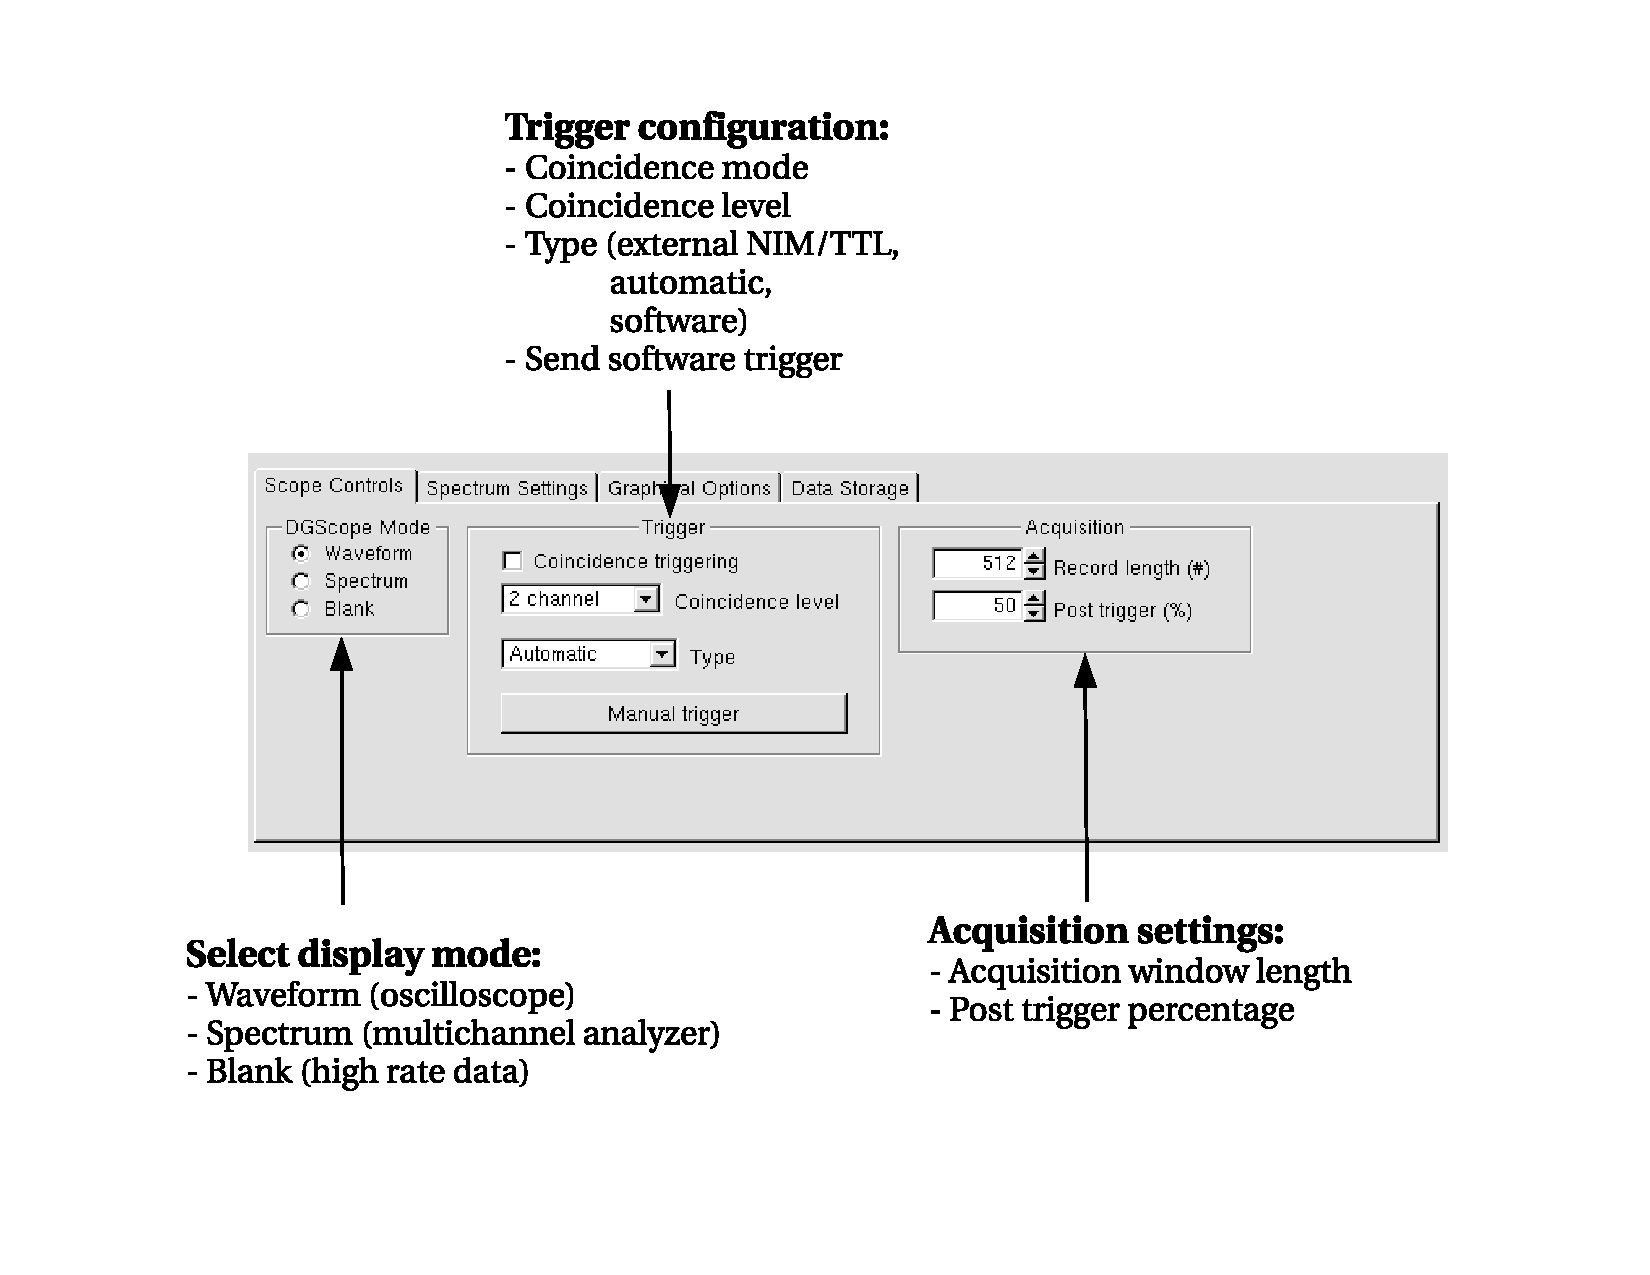
\includegraphics[width=6in]{images/OscilloscopeScope}
  \caption{An annotated close-up view of the ``Scope Controls'' subframe
    contained in the Oscilloscope frame. This subframe contains general
    settings that affect the global behavior of DGScope, such as what
    data to display, how to trigger the DGScope, and what the
    acquisition settings should be.}
  \label{fig:scopesubframe}
\end{figure}

\begin{figure}
  \centering
  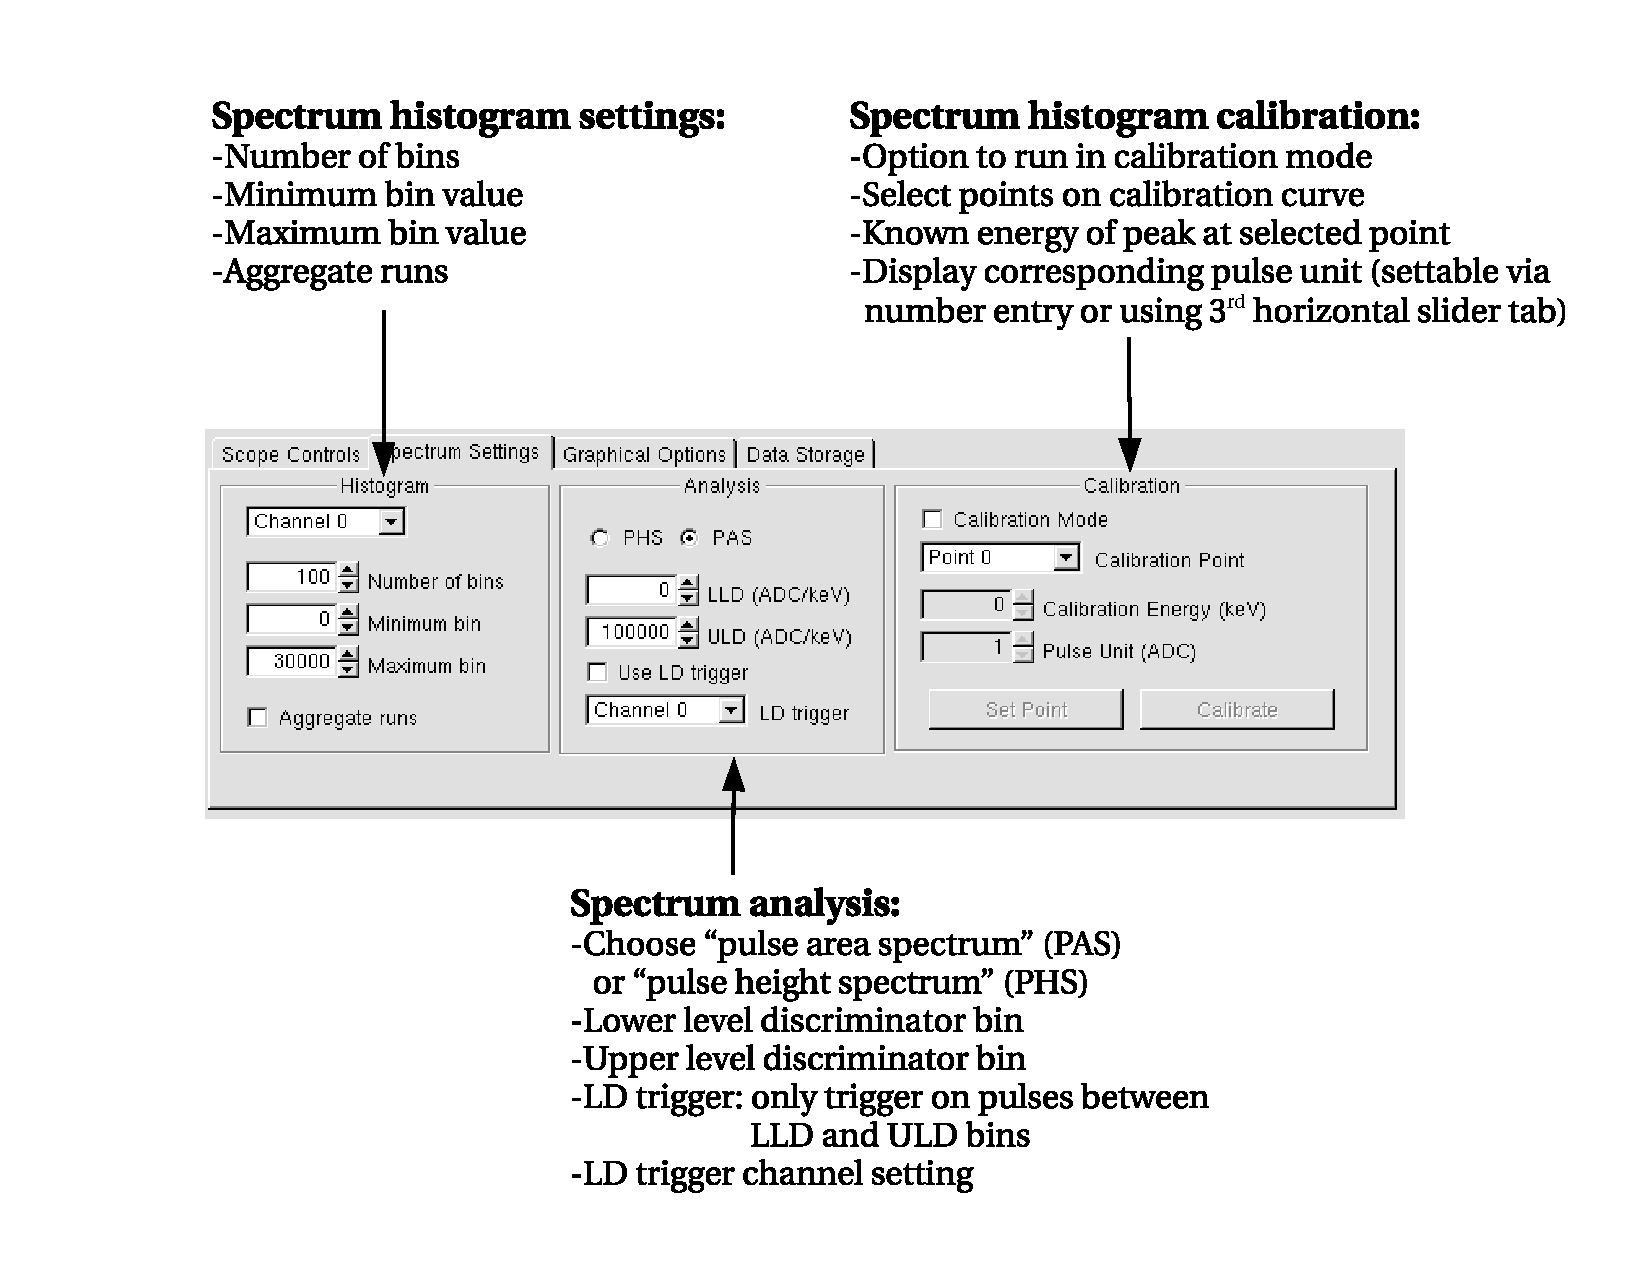
\includegraphics[width=6in]{images/OscilloscopeSpectrum}
    \caption{An annotated close-up view of the ``Spectrum Settings''
    subframe contained in the Oscilloscope frame. This subframe contains
    settings for how the acquired waveforms are analyzed and
    histogrammed to produce a pulse spectrum, as well as calibration
    settings for the spectrum.}
  \label{fig:spectrumsubframe}
\end{figure}


\begin{figure}
  \centering
  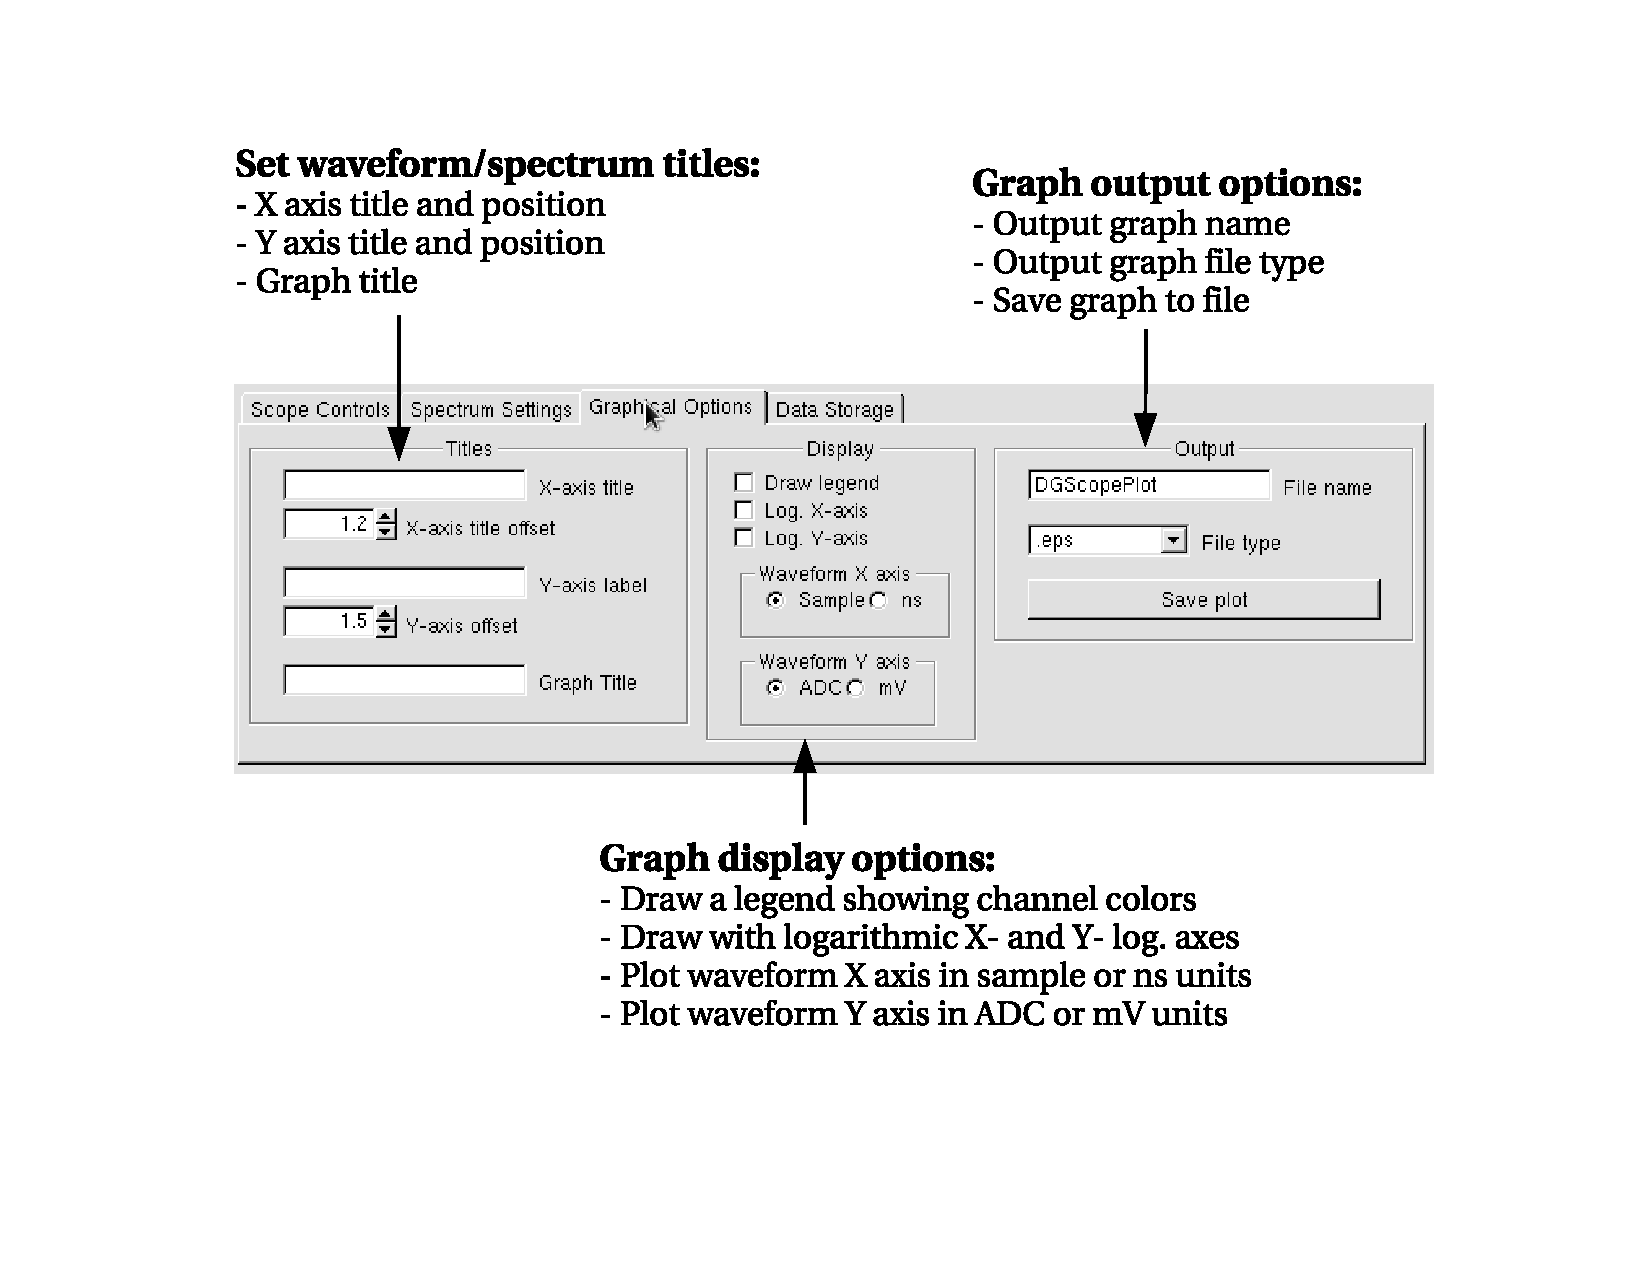
\includegraphics[width=6in]{images/OscilloscopeGraphical}
  \caption{An annotated close-up view of the ``Graphical Options''
    subframe contained in the Oscilloscope frame. This subframe contains
    settings for graphical control of the displayed data in DGScope,
    as well as options for save images of the displayed data to the
    hard drive.}
  \label{fig:graphicalsubframe}
\end{figure}

\begin{figure}
  \centering
  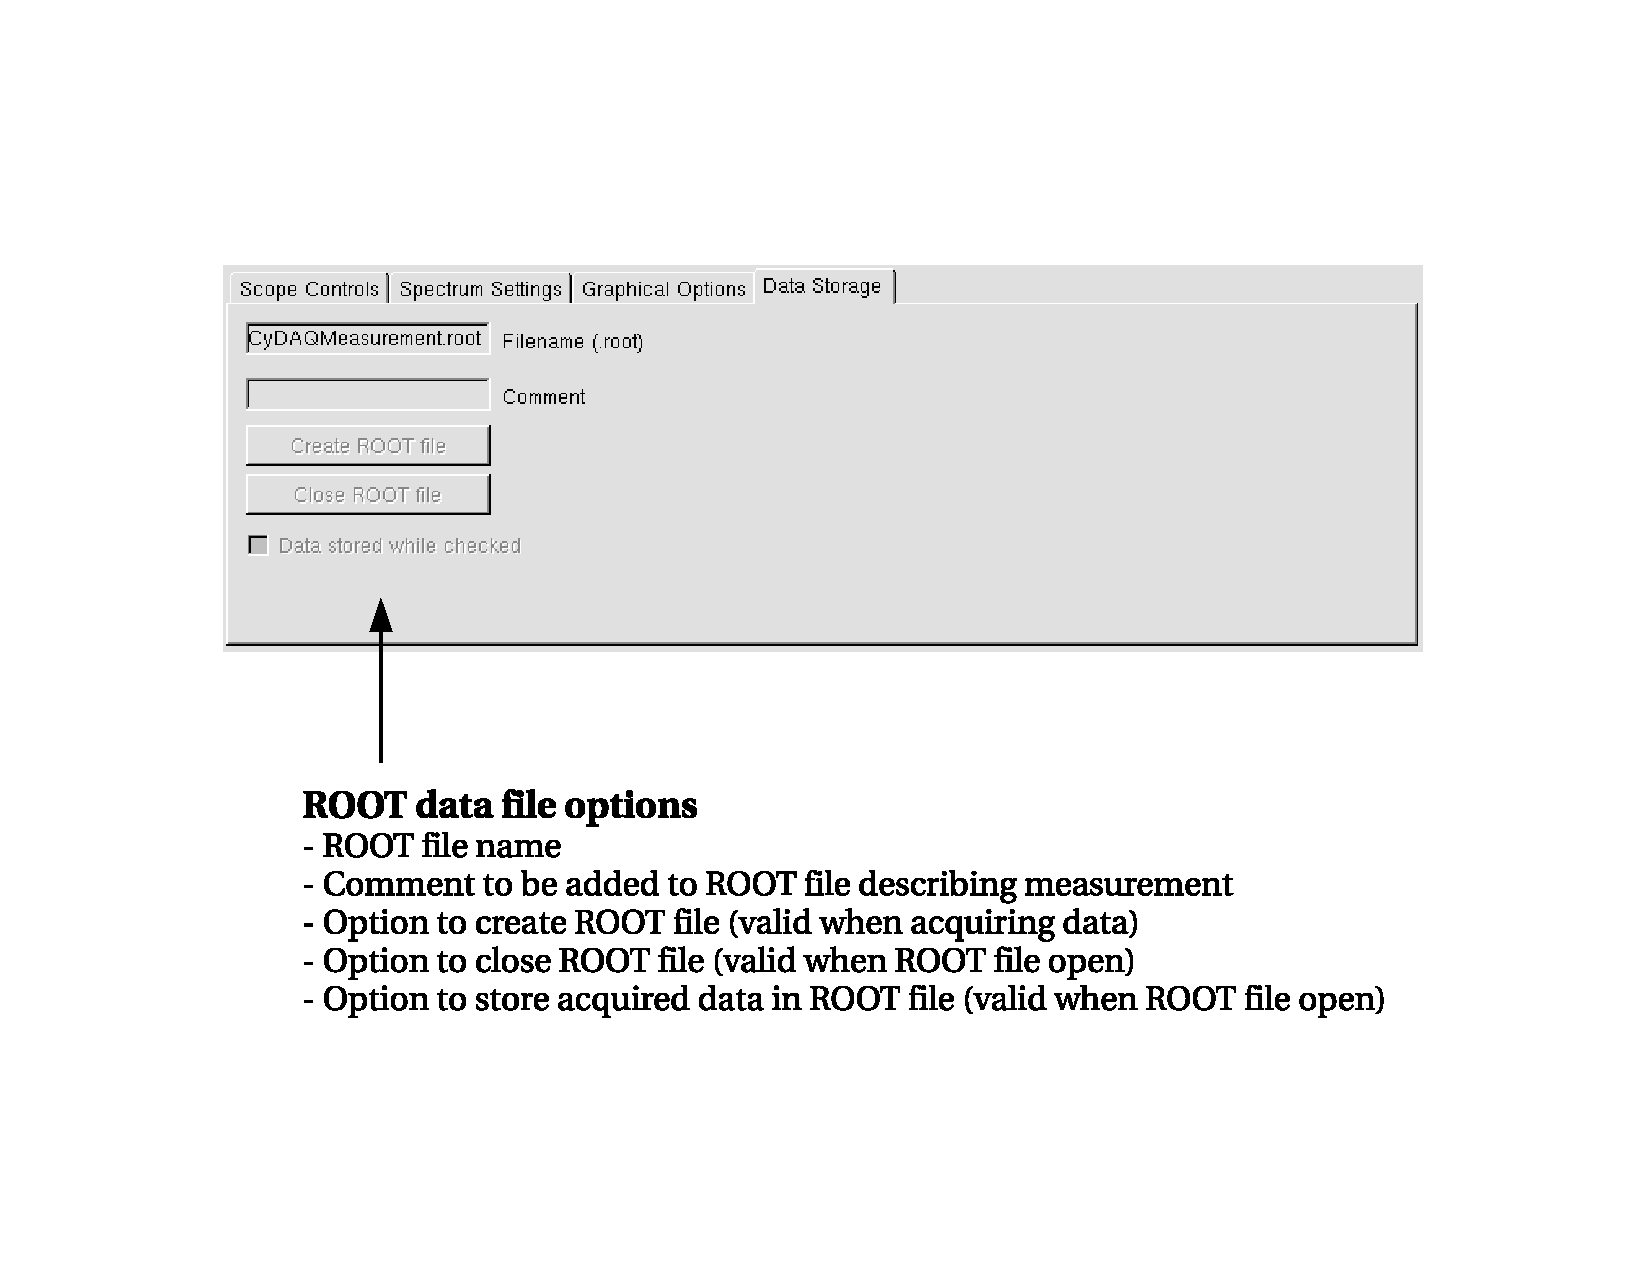
\includegraphics[width=6in]{images/OscilloscopeData}
  \caption{An annotated close-up view of the ``Data Storage'' subframe
    contained in the Oscilloscope frame. This subframe contains settings
    for persistent storage of the acquired waveform data in \ROOT
    files.}
  \label{fig:datasubframe}
\end{figure}

\begin{itemize}
  \item{\textbf{Channel Group Frame}: The 7 widgets contained in the
    channel group frame control channel-specific settings.
    \begin{itemize}
      \item{\textbf{Enable check button}: Enable/disable the digitizer
        channel. When enabled, signals input into the corresponding
        V1720 channel will be digitized, waveforms will be displayed
        in ``Waveform'' mode, and the waveforms will be processed into
        pulse spectra.}
      \item{\textbf{Pulse polarity radio buttons}: Used to indicate
        the direction of waveform rise relative to the signal
        baseline.``+'' indicates that the pulse rises above or to the
        positive side on the Y axis of the X axis baseline; ``-''
        indicates that the pulse rises below or to the negative side
        on the Y axis of the X axis baseline. While not necessary for
        plotting waveforms, pulse polarity is critical to the
        algorithms used to in the creation of pulse spectra.}
      \item{\textbf{Vert. Position number entry}: Sets the vertical
        position of the baseline relative to it's ``0'' position,
        i.e. a plotted offset of the input DC level of the
        baseline. This setting merely applies to the post-digitized
        \textit{plotted} waveforms and does not affect settings such
        as the trigger threshold, although the plotted trigger line
        will shift along with the channel baseline for
        consistency. This setting is primarily used to view multiple
        digitized waveforms simultaneously on the same DGScope
        canvas. Units of the settings are in ADC (analog-to-digital)
        units.}
      \item{\textbf{DC offset number entry}: Applies a DC offset to
        the input signal \textit{before} digitization such that the
        dynamic input range of the digitizer channel may be swung from
        -2--0 volts to 0--+2 volts. The input values are 16-bit
        integers in hex, such that 0x0000 corresponds to -2--0 volts,
        0x8000 corresponds to -1--+1 volt, and 0xffff corresponds to
        0--+2 volts. For details, please see the CAEN V1720 Digitizer
        Manual, Section XX, Page XX.}
      \item{\textbf{Trigger threshold number entry}: Sets the channel trigger
        threshold in ADC units. Waveforms that exceed this trigger
        will cause a global (all 8 channel) trigger-data acquisition
        cycle of the V1720 board when DGScope triggering is set to run
        in ``automatic'' mode.}
      \item{\textbf{Baseline min. and max. number entry}: Sets the
        range to use (from the minimum sample number to the maximum
        sample number) that is used for compute the average baseline
        value of the waveform. The range will be plotted on the
        DGScope when in ``Waveform'' mode as a shaded box in each
        channel's colors over the range used to calculate the
        baseline.}
    \end{itemize}
  }
  \item{\textbf{The Canvas Subframe}
    \begin{itemize}
      \item{\textbf{Double vertical slider}: The double vertical
        slider is used to control the Y axis zoom when DGScope is in
        either ``Waveform'' or ``Spectrum'' mode. The user may drag
        either end of the slider to zoom in or out, as well as
        dragging the entire slider by clicking-and-holding in the
        center of the slider to translate the view along the Y axis.}
      \item{\textbf{Triple vertical slider}; The triple vertical
        slider is used to control the X axis zoom when DGScope is in
        either ``Waveform'' or ``Spectrum'' mode. The user may drag
        either end of the slider to zoom in or out, as well as
        dragging the entire slider by clicking-and-holding in the
        center of the slider to translate the view along the X
        axis. In addition, the third slider tab that moves along the
        width of the slider body is used during calibration when
        DGScope is in ``Spectrum'' mode. For details on calibration,
        see Section~\ref{sec:calibration} of this manual.}
      \item{\textbf{Acquisition button}: the long button immediately
        underneath the X axis triple slider control the
        starting/stopping of data acquisition using DGScope. Initially
        red with text ``Stopped'', clicking the button will turn the
        button green and update the text to ``Acquiring'', indicating
        that DGScope is now acquiring and processing waveforms on the
        enabled digitizer channels. Clicking the button again will
        stop data acquisition and return the button to it's original
        state.}
    \end{itemize}
  }
  \item{\textbf{The Scope Controls subsubframe}: contains widgets that
    control global functionality of DGScope:
    \begin{itemize}
      \item{\textbf{DGScope Mode radio buttons}: sets the global
        function of DGScope. In ``Waveform'' mode, DGScope acts like a
        fully digital oscilloscope for visualization of input waveform
        from all enabled channels. In ``Spectrum'' mode, DGScope acts
        like an enhanced, fully digitial multichannel analyzer (MCA)
        plus computer, facilitating pulse spectra creation with
        different pulse processing algoriths. In ``Blank'' mode,
        nothing is plotted in DGScope, greatly reducing the CPU
        overhead of DGScope and making this mode extremely efficient
        for high-throughput data acquisition.}
      \item{\textbf{Coincidence Triggering check button}: when checked
        and DGscope is running in ``automatic'' triggering mode, a
        trigger is only generated if 2 or more channels have exceeded
        their respective channel trigger threshold and the waveforms
        overlap in time. For more details, see the CAEN V1720
        digitizer manual, Section XX, Page XX.}
      \item{\textbf{Coincidence Level selection box}: allows setting
        the coincidence level, i.e., the number of channels that must
        all exceed their respective trigger theshold to enable a
        trigger when DGScope is running in ``automatic'' mode and the
        ``coincidence trigger'' check button is enabled.}
      \item{\textbf{Trigger Type selection box}: allows setting the
        V1720 digiter to trigger in one of 3 modes. ``External''
        triggering mode generates global triggers on the rise of an
        input timing pulse, using either NIM fast logic or TTL fast
        logic signals. The NIM/TTL pulse must be fed into the external
        triggering input on the V1720 digitizer front panel via a LEMO
        00 connector on 50$\Omega$. ``Automatic'' triggering mode
        generates global triggers when one channel (or multiple
        channels if using coincidence triggering) exceeds its set
        trigger threshold. ``Software'' triggering mode generates a
        global trigger when the user clicks the manual trigger
        button.}
      \item{\textbf{Manual Trigger button}: Clicking the button
        generates a software trigger. When the triggering mode is set
        to ``software'', a global trigger is generated on the V1720
        digitizer.}
    \end{itemize}
  }
\item{\textbf{The Spectrum Settings subframe}: contains widgets that
    control the behavior of the pulse spectra:
    \begin{itemize}
    \item{\textbf{Histogram channel selection box}: Select which
        enabled channel's pulse spectra histogram will be plotted in
        the DGScope canvas. At present, only one channel can be
        plotted at a time, although the user may switch between
        channels during acquisition.}
    \item{\textbf{Number of bins number entry}: Select the number of
        bins used in the pulse spectra histogram}
    \item{\textbf{Mininmum and maximum bin number entries}: Set the
        minimum and maximum bin values of the pulse spectra histogram}
    \item{\textbf{PHS and PAS radio buttons}: Select whether pulse
        height (PH) or pulse area (PA) algorithms will be used to
        produced pulse spectra (S) from digitized waveforms.}
    \item{\textbf{LLD and ULD number entries}: Set the lower level
        discriminator (LLD) and upper level discriminator (ULD)
        values. Waveforms with pulse height/area that are below the
        LLD or above the ULD are not histogrammed into the spectrum.}
    \item{\textbf{Use LD trigger check box}: Use the LLD/ULD values
        from one channel (see next widget description) as a
        ``trigger'' for saving digitizer waveforms to an open \ROOT
        file. The purpose is to ``trigger'' only on pulses between
        known pulse (energy) bins.}
    \item{\textbf{LD trigger selection box}: Select the channel that will be used
        for level discriminator (LD) triggering. Note that when this
        channel triggers, i.e. that analyzed waveform falls between
        the LLD and ULD bin values, a global trigger is generated that
        triggers all 8 V1720 digitizer channels.}
    \item{\textbf{Calibration mode check box}: When checked and
      DGScope is running in ``spectrum'' mode, the user may calibrate
      the pulse spectrum to convert the X axis of the spectrum from
      ``pulse units'' in ADC to ``energy units'' such as keV.}
    \item{\textbf{Calibration point selection box}: Selects the
      calibration point to be set. The number of selection options
      starts at 0 and increases by 1 each time the user adds a point
      to the calibration by clicking the ``Set Point'' button.}
    \item{\textbf{Calibration energy number entry}: Enter the known
      particle energy in keV corresponding to a peak in the present
      spectrum, which has the third horizontal slider tab centered on
      it or which will have its pulse unit entered in the ``Pulse
      Unit'' number entry.}
    \item{\textbf{Pulse unit number entry}: Should be set to the
      center value of a peak in the pulse spectrum that represents the
      known particle energy entered in the ``Calibration energy''
      number entry widget. The pulse unit will be automatically set
      (and this number entry updated) when the user drags the third
      horizontal slider tab to center the vertical dashed red line
      (which will appear on the DGscope canvas) on the peak in the
      spectrum.}
    \item{\textbf{Set point button}: Sets the current calibration
      point selected in the Calibration Point selection box. Clicking
      the button assigns the energy and pulse unit values to a point
      on the calibration curve, which is an energy vs. pulse unit
      curve for converting the pulse spectrum to an energy
      spectrum. After this button is clicked, a new calibration point
      will appear in the Calibration Point to continue adding points
      to the calibration curve.}
    \item{\textbf{Calibrate button}: Uses all of the set calibration
      points to create a calibration curve. Once this button is
      clicked and the Calibration Mode check box in unchecked, the
      calibration curve is used to histogram all analyzed waveforms
      (pulse height or pulse area values in ADC) into an energy
      spectrum, where the bin values now represent particle energy in
      keV.}
    \end{itemize}
    }
  \item{\textbf{Graphical Options}: contains widgets that control the
    appearance of what is plotted on the DGScope canvas:
    \begin{itemize}
      \item{\textbf{X-axis title text entry}: Sets the title of the
        X-axis for both the waveform and spectrum plot.}
      \item{\textbf{X-axis title offset text entry}: Sets the position
        of the X-axis title below the X-axis labels.}
      \item{\textbf{Y-axis title text entry}: Sets the title of the
        Y-axis for both the waveform and spectrum plot.}
      \item{\textbf{Y-axis title offset text entry}: Sets the position
        of the Y-axis title below the Y-axis labels.}
      \item{\textbf{Graph title text entry}: Sets the title of the
        DGScope graph.}
      \item{\textbf{Draw legend check box}: If checked, draws a legend
        on the waveform plot showing the channel-to-color mapping.}
      \item{\textbf{Log. X-axis / Log. Y-axis check boxes}: If
        checked, will display the X-axis / Y-axis in logarithmic
        scale. Can be freely switched during data taking.}
      \item{\textbf{Waveform X-axis radio buttons}: Will display the
        X-axis for waveform plotting in units of Sample (recall that a
        sample is taken every 4 nanoseconds with the V1720 digitizer)
        or nanoseconds (``ns''). Can only be set when DGScope is not
        acquiring data.}
      \item{\textbf{Waveform Y-axis radio buttons}: Will display the
        Y-axis for waveform plotting in units of ADC (integer
        analog-to-digital units, 0 being the minimum and 4095 begin
        the maximum) or millivolts (``mV''). Can only be set when
        DGScope is not acquiring data.}
      \item{\textbf{Output file name text entry}: Sets the name of the
        image file that will contain the current contents of the
        DGScope canvas.}
      \item{\textbf{Output file type selection box}: Sets the file
        type for the image file: .eps, .ps, .png, .jpeg image formats
        are current supported. But please, be a professional and use
        .eps. Vector graphics are the only way to go! No one wants to
        see a rastered image in a professional report.}
      \item{\textbf{Save plot button}: Saves the contents of the
        DGScope canvas as they currently appear to the file name and
        format set in the previous widgets. Can be clicked while
        DGScope is acquiring data. In addition, all file output names
        end in an integer that is incremented if the user attempts to
        create image files of the same name.}
    \end{itemize}
  }
  \item{\textbf{Data Storage}: contains widgets that control
    persistent storage of digitized waveforms in \ROOT files:
    \begin{itemize}
      \item{\textbf{Filename text entry}: Sets the name of the \ROOT
        file to be opened for receiving digitized waveforms. The name
        should (by convention) end in the .root extension to ease file
        identification for yourself and other users.}
      \item{\textbf{Comment text entry}: Allows the user to entry
        anything he/she wants to be stored in the \ROOT file. Entries
        could describe the current measurement, parameters, notes,
        ideas, or nice compliments about the author of this manual.}
      \item{\textbf{Create \ROOT file button}: When DGScope is
        acquiring data and this button is clicked, the \ROOT file
        (name set in the previous widget) will be created on the hard
        drive. This widget is disabled when DGScope is not acquiring
        data. Note that an error message will be printed to the
        terminal from which \ADAQ was executed if the
        user tries to create a \ROOT file with the same name as an
        existing \ROOT file. Note also that, while the file is opened
        and some measurement data has been written to the \ROOT file,
        waveforms are not stored in the file until the Data storage
        check button is engaged.}
      \item{\textbf{Close ROOT file button}: Closes the currently open
        \ROOT file. Before the file closes, all required \ROOT
        operations are performed to ensure all waveform data and
        structures within the file are written correctly.}
      \item{\textbf{Data stored when checked button}: When this button
        is checked, waveforms are written to the currently open \ROOT
        file.}
    \end{itemize}
  }
\end{itemize}
    
    
\section{Persistent data storage in \ROOT files}
\label{sec:datastorage}
This section describes how \ADAQ stores data in \ROOT
files, which is critical to understand how to use offline analysis
codes to extract the data from the \ROOT files and analyze it. An
understanding of C++ programming and object-orienting principles are
helpful but not required to grasp the essentials of this section.

\subsection{The \ROOT file}
A complete description of what a \ROOT file is outside of the scope of
this manual\footnote{The interested user can find all the gory details
  in chapter 11 of the \ROOT manual:
  \purl{http://root.cern.ch/download/doc/ROOTUsersGuideHTML/ch11.html}};
however, a simple description is that a \ROOT file is like a unix
directory, in that it can contain unlimited further directories,
files, objects, etc, all in a machine-independent format for
portability.

\lstset{
  language=C++, 
  basicstyle=\footnotesize, 
  numbers=left,
  numberstyle=\footnotesize,
  numbersep=0pt
}

The \ROOT file format created by \ADAQ is relatively
simple and  contains only three objects:
\begin{itemize}
  \item{A class object of type \texttt{CyDAQRootMeasParams}, which is
    a custom-defined C++ class that contains the value of each
    channel's settings during a measurement and the RecordLength
    (acquisition window width) as member data. The class declaration
    for \texttt{CyDAQRootMeasParams} is:
    \begin{lstlisting}
      class CyDAQRootMeasParams : public TObject{

        public:
        std::vector<double> DetectorVoltage;
        std::vector<double> DetectorCurrent;
        std::vector<double> DCOffset;
        std::vector<double> TriggerThreshold;
        std::vector<double> BaselineCalcMin;
        std::vector<double> BaselineCalcMax;
        
        int RecordLength;
        
        ClassDef(CyDAQRootMeasParams,1);
      };
    \end{lstlisting}
    As can be seen on line 1, the class inherits from a \ROOT
    \texttt{TObject} class, which helps it seamlessly interface with
    the \ROOT file and \ROOT offline data analysis code. Lines 4--9
    show that one C++ standard library \texttt{vector} container is
    used to store a single type of channel parameter; thus, each
    vector will have 8 entries corresponding to the 8 V1720 digitizer
    channels. Line 11 shows the RecordLength is simply an
    integer. Finally, Line 13 simply declares the class to \ROOT.
  }
  \item{a class object of type \texttt{TObjString}, which is a \ROOT
    class that represents a string. It is used to store whatever
    additional information the user would like to have attached to the
    data contained in the \ROOT file as a string.}
  \item{A \ROOT \texttt{TTree} that contains all of the digitized
    waveforms. A \texttt{TTree} is essentialy a hierarchical structure
    for logically categorizing and efficiently storing large
    quantities of data. Here, the tree is subdivided into 8
    ``branches'' (one for each V1720 digitizer channel) that holds the
    digitized waveforms as C++ standard library \texttt{vector}
    objects of length ``RecordLength''. Theoretically, an unlimited
    number of \texttt{vector} objects representing digitized waveforms
    can be stored on each channel's branch.}
\end{itemize}

While \ADAQ is actively acquiring data, the user has
the option to create a new \ROOT file on the ``Data Storage'' subframe
on the ``Oscilloscope'' frame. The act of clicking the ``Create ROOT
File'' button performs the following actions:
\begin{itemize}
  \item{creates the user-named \ROOT file on the harddisk}
  \item{creates the three objects described above in the active
    instance of \ROOT's memory. The three class objects, rather than
    being located on the harddisk are located on the \ROOT file
    (recall that it acts like a unix directory).}
  \item{assigns values of the \texttt{CyDAQRootMeasParams} object and
    the \texttt{TObjString} by obtaining the values from the
    appropriate \ADAQ widgets}
\end{itemize}

When the user has clicked the ``Data stored while checked'' check box
having opened a \ROOT file, digitized waveforms are actively written
to the \ROOT \texttt{TTree} object. The user can verify this by
continuously inspecting the size of the \ROOT file, which will grow in
size as waveforms are written to the \ROOT \texttt{TTree} object
contained on the \ROOT file. 

Finally, when the user is done acquiring data and clicks the ``Closed
ROOT file'' button, the three objects are finalized on the \ROOT file
(``written to the ROOT file'' in the \ROOT parlance) and a number
\ROOT protocol operations are performed to finalize the format of the
\ROOT file before it is closed.



    
    




\include{tutorial1}
\chapter{Tutorial 2: Saving digitized waveforms to a \ROOT file}
\label{chap:tutorial2}
This chapter provides a detailed, step-by-step tutorial that covers
using \ADAQ to store digitized detector waveforms into a \ROOT file.

The user is expected to have covered Tutorial 1 before beginning this
tutorial, as a number of important skills taught there are critical to
this tutorial as well.

\section{Assumptions}
\label{sec:assumptions2}
The assumptions for this tutorial are identical to those found in
Tutorial 1. Please see Section~\ref{sec:assumptions1}.

\section{Hardware setup}
\label{sec:hardwaresetup2}
The hardware setup for this tutorial is identical to that found in
Tutorial 1. Please see Section~\ref{sec:hardwaresetup1}

\section{Configure \ADAQ for acquisition}
\label{sec:configure2}

\section{Acquiring waveforms}
\label{sec:acquiring2}
Setting up waveform acquisition is identical to that found in Tutorial
1. Please see Section~\ref{sec:acquiring1}.

\section{Saving waveforms  into a \ROOT file}
The section describes the steps to create a \ROOT file, store
digitized waveforms in it, and successfully close the \ROOT file.
At this point in the tutorial

\begin{enumerate}
  \item{Configure all waveform acquisition settings to their desired
    value using the channel 0 specific settings found towards the
    top-right of the Oscilloscope frame. When done adjusting channel
    0's settings, stop the acquisition.}
  \item{Click the ``Data Storage'' subtab toward the bottom right of
    the Oscilloscope frame. Note that all the widgets on this
    subframe are disabled.}
  \item{Start the acquisition. Note that ``Filename'', ``Comment'',
    and ``Create ROOT File'' widgets are enabled, indicating that
    these widgets may only be used when acquisition is running.}
  \item{Set the \ROOT filename. Note that the user is responsible to
    providing an appropriate suffix, with ``.root'' being the
    recommended value. When done, click the ``Create ROOT File''
    button. This creates and initializes the \ROOT file on the hard
    disk, as well as enables the ``Close ROOT file'' and ``Data stored
    ...'' check box, since the \ROOT file is now open and can receive
    data. Note that at this point no waveforms are being written to
    the \ROOT file even though waveforms are being acquired by
    \texttt{|CyDAQRootGUI}.}
  \item{Click the ``Data stored ...'' check box at the bottom of the
    subframe. The digitized waveforms on channel 0 that appear on the
    DGScope canvas are now being written to the \ROOT file. The user
    may continually view the size of the created \ROOT file to
    convince him- or herself that the \ROOT file is receiving data and
    growing in size.}
  \item{Once it is determined that sufficient data has been acquired
    (by viewing and being satisfied with a pulse spectrum or
    completing a 5 minute data acquisition session, for example),
    uncheck the ``Data stored ...'' check box. Waveforms have ceased
    to be written to the \ROOT file; the \ROOT file is still open and
    must be closed correctly to ensure the file is not corrupted.}
  \item{Click the ``Close ROOT File'' button. This performs a number
    of final, required operations on the \ROOT file and closes it.}
\end{enumerate}

At this point in the tutorial, a complete \ROOT file exists on the
hard disk containing digitized waveforms and can be processed with
offline data acquisition code. The user may now: create a new \ROOT
file and repeat the above steps; cease acquisition, modify channel
settings and repeat the above steps; or move on to a completely
different task.

\section{Offline analysis using the \ROOT file}
The \ADAQ user is responsible for developing his or her own code that
will be used offline to process the data contained in the \ROOT
file. To guide the user in creating his or her own analysis code, a
data analysis ``template'' has been created that explicitly shows the
user how to:
\begin{itemize}
  \item{create a standalone, C++ and \ROOT based offline analysis code}
  \item{open a \ADAQ \ROOT file and extract the V6534 and V1720 channel parameters}
  \item{extract the digitized waveforms into C++ integer arrays for processing}
\end{itemize}
The template is configured to open a \ROOT file (the path to the file
must be specified on the command line), print the V6534 and V1720
channel parameters, and the cycle through all of the V1720 channel 0
waveforms contained in the \ROOT file.

The user should copy the template directory to a new directory, and
use it as the basis for his or her own analysis code. All of the
critical interactions with the \ROOT file that must be performed to
extract all stored data are explicitly shown and heavily commented,
providing the user with a good understanding of the steps as well as a
solid foundation for his or her own analysis code. The template code
may be found in the \texttt{\$CYDAQHOME/analysis/analysisTemplate/}
directory.

\section{Conclusion}
Congratulations! If you have reached this point without throwing
errors or cursing the author with reckless abondon, you have
successfully used \ADAQ to acquire detector waveform data and store it
in a \ROOT file for permament storage and offline data analysis. The
interested user is recommended to repeat this tutorial but explore the
numerous \texttt{CyDAQRootGUI} settings that were not used in this
tutorial, especially acquiring data in coincidence and using the level
discrimanator settings as the ``trigger'' for storing waveforms in the
\ROOT file.



\end{document}
